This section present an analysis of the microstructure based on the pair probability density function  $P_\text{nst}(\textbf{x},\textbf{r},t)$.
After identifying the different forms of the microstructure with respect to the dimensionless parameters, we introduce a general and concise way to quantify it.

\subsection{Nearest pair distribution function}
In this section, only the relative position between pairs will be of interest. 
Therefore, we introduce the reduced probability distribution,
\begin{equation*}
    P_\text{nst}(\textbf{x},\textbf{r},t)
    = \int_0^\infty P_\text{nst}(\textbf{x},\textbf{r},t,a) da.
\end{equation*}
In the following graphs, we assume an axis symmetry with respect to the vertical axis due to the periodic boundary of the numerical domain.
Therefore, the coordinate \textbf{r} can be represented by its radial and azimuthal components, $r = |\textbf{r}|$ and $\theta$, respectively.
Where $\theta$ is the angle between the vector \textbf{r} and the vertical direction.
Consequently, In the following, we analyze the weighted probability density function $P_\text{nst}^n$ in a spherical coordinate frame, defined as follows:
\begin{equation*}
    P_\text{nst}^n(\textbf{x},t,r,\theta)
    =\frac{1}{2\pi \sin\theta r^2 dr d\theta n_p(\textbf{x},t) }\int_0^\infty P_\text{nst}(\textbf{x},t,r,\theta,a) da.
\end{equation*}


\subsubsection*{Low inertial effects }
We begin with a detailed analysis of $P_\text{nst}^n$ at low Galileo numbers to investigate the influence of $\lambda$ and $\phi$ on the microstructure when inertia has a negligible effect.
As it will be seen in the next section the nearest particle statistic isn't necessarily fore-after symmetric with respect to the horizontal plane, as it would be the case for a pair statistic average. 
Nevertheless, it turns out that $P_\text{nst}$ possesses a nearly symmetric distribution, such that $P_\text{nst}^n(\textbf{x},t,r,\theta)\approx P_\text{nst}^n(\textbf{x},t,r,- \theta)$. 
Therefore, in the following histograms, displayed in \ref{fig:Pnst_low_Ga} and \ref{fig:Pnst_high_Ga}, we choose to show only the upper part of the distribution.
\begin{figure}[h!]
    \centering
    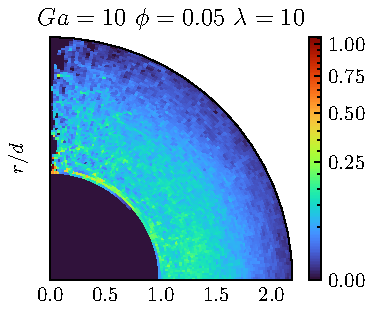
\includegraphics[height=0.21\textwidth]{image/HOMOGENEOUS_NEW/Dist/Pnst_l_10_Ga_10_PHI_0_05.pdf}
    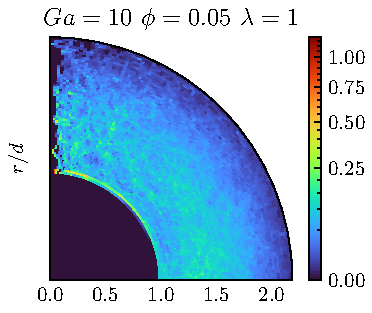
\includegraphics[height=0.21\textwidth]{image/HOMOGENEOUS_NEW/Dist/Pnst_l_1_Ga_10_PHI_0_05.pdf}
    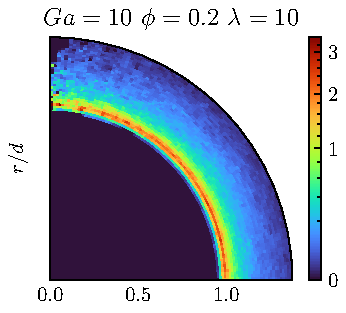
\includegraphics[height=0.21\textwidth]{image/HOMOGENEOUS_NEW/Dist/Pnst_l_10_Ga_10_PHI_0_2.pdf}
    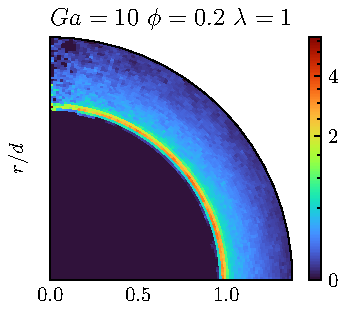
\includegraphics[height=0.21\textwidth]{image/HOMOGENEOUS_NEW/Dist/Pnst_l_1_Ga_10_PHI_0_2.pdf}
    \caption{Histogram of the normalized probability density function $P_\text{nst}^n$ at low inertial effects $Ga = 10$.
    The color map represents the values of $P_\text{nst}^n$.
    The origin corresponds to the position of the test particle.
    The dimensionless radial and azimuthal coordinates, $|\textbf{r}|/d$ and $\theta$, correspond to the nearest neighbor position.
    The vertical direction corresponds to the flow direction, which is also the axis of symmetry for $P_\text{nst}^n$.
    (left) Low volume fraction cases $\phi=0.05$ for $\lambda = 1,10$.
    (right) High volume fraction cases $\phi=0.1$ for $\lambda = 1,10$ }
    \label{fig:Pnst_low_Ga}
\end{figure}
The first observation from \ref{fig:Pnst_low_Ga} indicates that the likelihood of finding the nearest neighboring particle at an angle $\theta$ is uniform across all $\theta$.
This suggests that $P_\text{nst}^n$ is isotropic at these \textit{Galileo} numbers. 
If we compare the low volume fraction case to the high volume fraction case, we can observe that $P_\text{nst}^n$ is more concentrated near the contact of the particles ($r = 2a$) in the latter case.
This fact has already been observed for solid particles, we will see in the following that it is even accentuated for higher inertial effects. 
Regarding the impact of the viscosity ratio, $P_\text{nst}^n$ appears quite similar for both values of $\lambda$. 
For instance, $\lambda$ seems to have no impact on the suspension microstructure.
